\documentclass{article}
\usepackage[utf8]{inputenc}
\usepackage[T1]{fontenc}
\usepackage{hyperref}
\hypersetup{colorlinks=true, linkcolor=blue, filecolor=magenta, urlcolor=cyan,}
\urlstyle{same}
\usepackage{amsmath}
\usepackage{amsfonts}
\usepackage{amssymb}
\usepackage[version=4]{mhchem}
\usepackage{stmaryrd}
\usepackage{graphicx}
\usepackage{caption}
\usepackage{subcaption}
\usepackage{placeins}
\usepackage[
    top=1in,
    bottom=1in,
    left=1in,
    right=1in
]{geometry}
\begin{document}

\section*{AM16 Final Exam}

\section*{1 Problem (115 points)}

\subsection*{(a) Data Visualization}

\paragraph{Data Loading and Preprocessing.}
In this problem, we work with real weather data from \texttt{NETCDF4} files for the years 1979, 1980, 1981, 1983, and 1985. Each file contains the variable \(\mathbf{z}\) with dimensions \(\text{time} \times \text{channel} \times \text{latitude} \times \text{longitude}\), sampled every 6 hours. We load the data, select the variable \(\mathbf{z}\), and convert it into a \texttt{numpy} array.

Before any modeling, we apply normalization. Specifically, we compute
\[
\mu = 126{,}784.01, \quad \sigma = 72{,}895.65
\]
from the training years (1979, 1980, 1981, 1983) and then transform all data as:
\[
z_{\text{norm}} = \frac{z - \mu}{\sigma}.
\]
This step ensures that the neural networks train more stably and that all channels share a comparable scale.

\paragraph{Data Visualization.}
To get a feel for what our data looks like, we plot contour maps over latitude and longitude. at select time steps (indices 0, 365, 730, 1095, 1459) These indices roughly correspond to days 0, 91, 182, 273, and 365:

\begin{figure}[h]
    \centering
    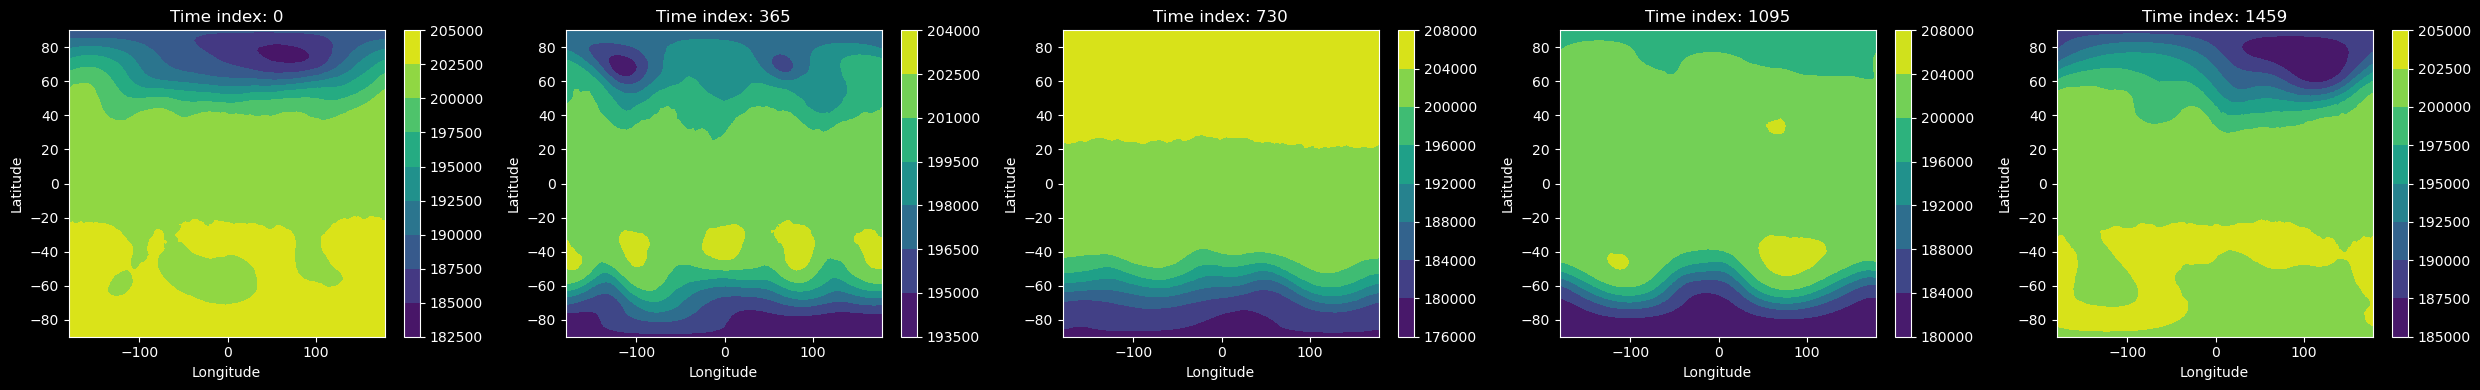
\includegraphics[width=0.9\textwidth]{../plots/visualized_data.png}
    \caption{Visualization of weather data spatial patterns at selected time steps showing the evolution of weather patterns across different temporal points.}
    \label{fig:weather_vis}
\end{figure}

\subsection*{(b) Denoising Variational Autoencoder}

In part (b), we develop a \textbf{convolutional denoising variational autoencoder (VAE)} to reconstruct the weather data from corrupted inputs.

\paragraph{Data Corruption.}
To simulate sparse data, we randomly zero out a fraction \(k\)\% of the grid points in each time step. We consider \(k \in \{30, 60, 90\}\). The corruption is applied to both training and testing data.

\paragraph{VAE Architecture.}
\begin{itemize}
    \item \textbf{Encoder:} A stack of four 2D convolutional layers, each with kernel size \(3 \times 3\), stride \(2\), and \texttt{LeakyReLU} activations. After passing through these layers, the representation is mapped to a latent space of dimension 128. We parameterize \(\mu\) and \(\log\sigma^2\) in this latent space.
    \item \textbf{Decoder:} Mirrors the encoder with transposed convolutions, again with \texttt{LeakyReLU}. It reconstructs the original spatial dimensions and channel count. 
\end{itemize}

\paragraph{Loss Function.}
We minimize the standard VAE loss, which is a sum of:
\[
\mathcal{L} = \underbrace{\mathrm{MSE}\bigl(x_{\text{true}}, x_{\text{recon}}\bigr)}_{\text{reconstruction loss}}
\;+\;\underbrace{\beta \,\mathrm{KL}\bigl(q(\mathbf{z}|\mathbf{x}) \,\|\, p(\mathbf{z})\bigr)}_{\text{KL divergence}}.
\]
where, \(\beta\) is a weight. We choose MSE because our data is continuous. The KL term regularizes the latent space to remain close to a standard Gaussian.

\paragraph{Training Details.}
\begin{itemize}
    \item \textbf{Optimizer:} Adam with a learning rate of \(0.001\) that drops to \(0.0001\) if the validation loss plateaus.
    \item \textbf{Epochs:} 20 epochs for each corrupted sample, plus a shorter 7 epochs on clean training data to fine tune. which results in 67 total epochs
    \item \textbf{Batch Size:} 16
    \begin{figure}[ht]
        \centering
        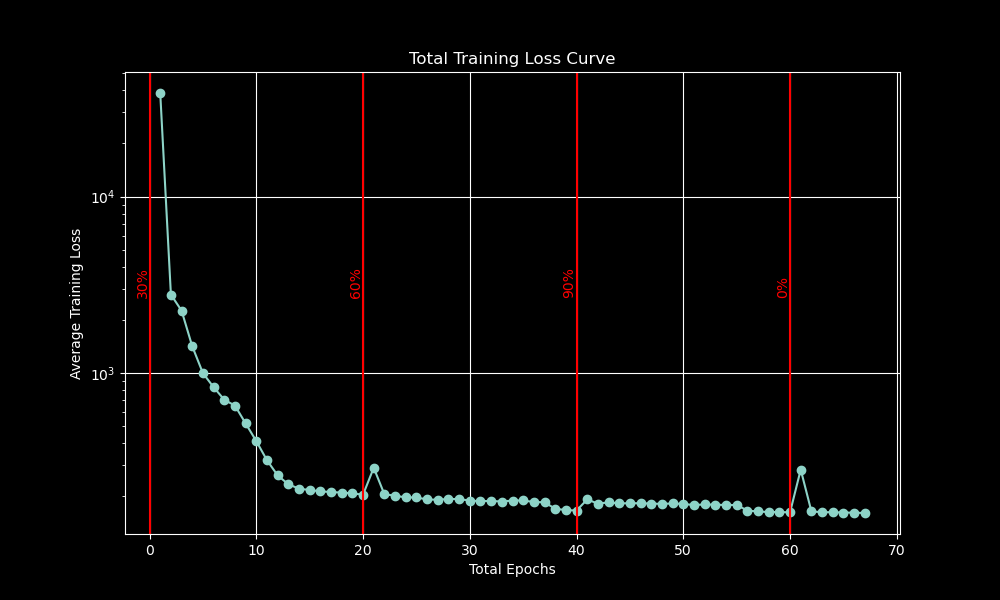
\includegraphics[width=0.6\textwidth]{../loss/full_loss_curve20250320-223912.png}
        \caption{Training loss curve for the denoising VAE with each training phase marked}
        \label{fig:vae_loss}
    \end{figure}
\end{itemize}

\paragraph{Evaluation.}
We test on year 1985. For each sparsity level (30\%, 60\%, 90\%), we visualize the predictions, Our MSE values for the chosen time step are: 0.00026 for 0\% sparsity, 0.00032 for 30\% sparsity, 0.00031 for 60\% sparsity, and 0.00033 for 90\% sparsity

\begin{figure}[h]
    \centering
    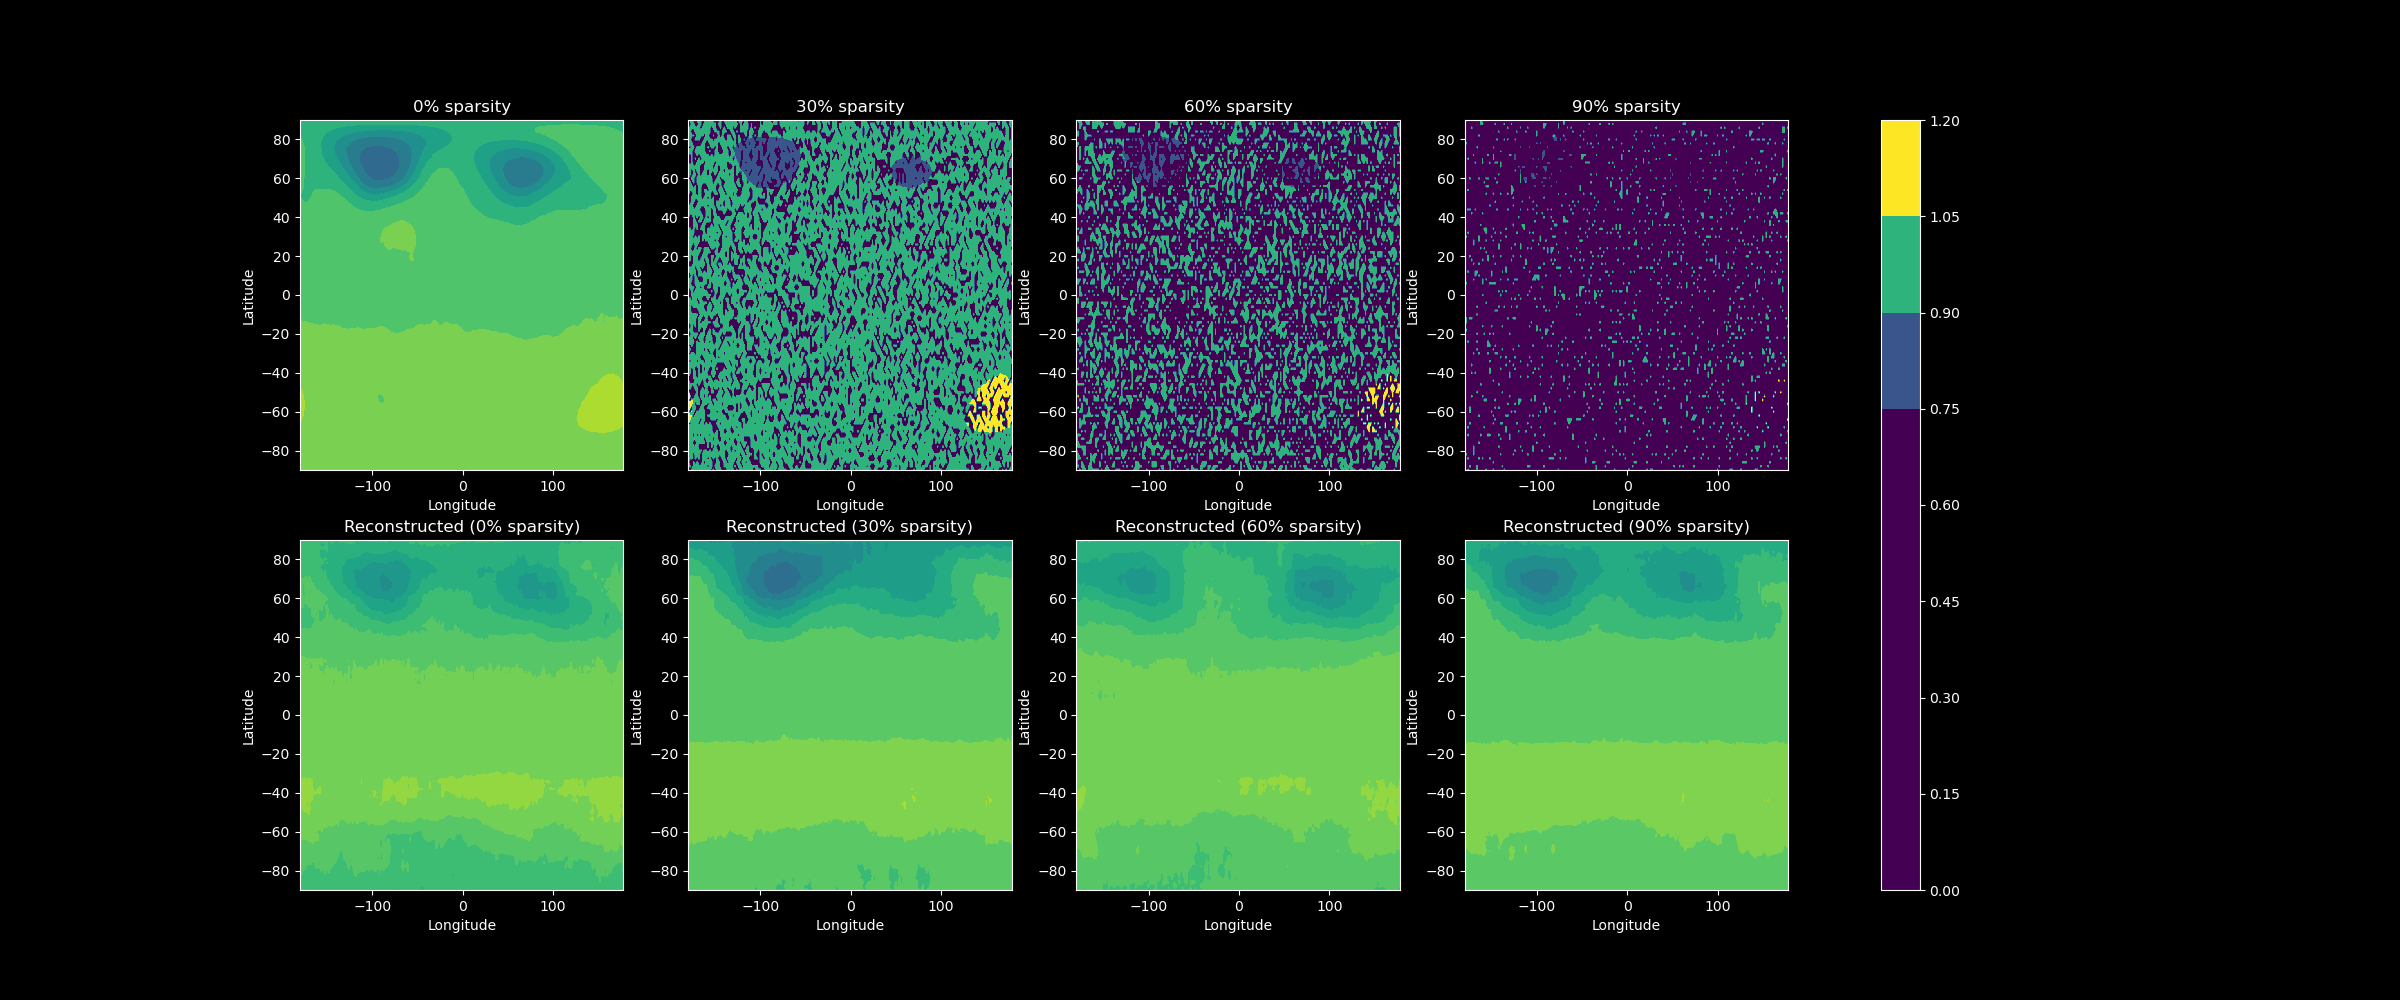
\includegraphics[width=0.6\textwidth]{../plots/reconstruction_comparison20250320-223912.png}
    \caption{Denoising VAE reconstruction for 1985 at 0\%, 30\%, 60\%, and 90\% sparsity., compared to with the noised input.}
    \label{fig:vae_preds}
\end{figure}

\FloatBarrier
\newpage
\section*{2 Problem (15 points)}

\subsection*{Conditional VAE for Autoregressive Prediction}

\paragraph{Data Pairing and Preprocessing:}
First we apply the same conditioning as we do for the denoising VAE.
then we form \((X(t), X(t+1))\) pairs from the training years. Each \(X(t)\). For each pair, \(X(t)\) is the \textit{condition} and \(X(t+1)\) is the \textit{target}.

\paragraph{Model Architecture:}
We design a conditional convolutional VAE with a similar Architecture to the Denoising mode, with two encoders:
\begin{enumerate}
    \item An encoder for the target \(X(t+1)\), producing \(\mu\) and \(\log\sigma^2\) in latent space.
    \item A simpler encoder for the condition \(X(t)\), producing a condition embedding.
\end{enumerate}
We concatenate the latent sample from the first encoder with the condition embedding from the second, then pass this into a decoder (similar convolutional structure as in part (b)) to reconstruct \(X(t+1)\).

\paragraph{Loss Function.}
Again, we use
\[
\mathcal{L} = \mathrm{MSE}\bigl(X(t+1)_{\text{true}}, X(t+1)_{\text{pred}}\bigr) \;+\; \beta \,\mathrm{KL}\bigl(q(\mathbf{z} | X(t+1)) \,\|\, p(\mathbf{z})\bigr).
\]
Here, the condition embedding from \(X(t)\) acts as additional input to the decoder, making the model \emph{conditional} on the previous time step.

\paragraph{Training Details.}
\begin{itemize}
    \item \textbf{Optimizer:} Adam, learning rate 0.001 dropping first to 0.0001 and then to 0.00005, if it encounters plateaus, we'll train for 50 epochs
    \item \textbf{Implementation:} Provided in \texttt{train\_cond\_vae.py}.
\end{itemize}

\begin{figure}[ht]
    \centering
    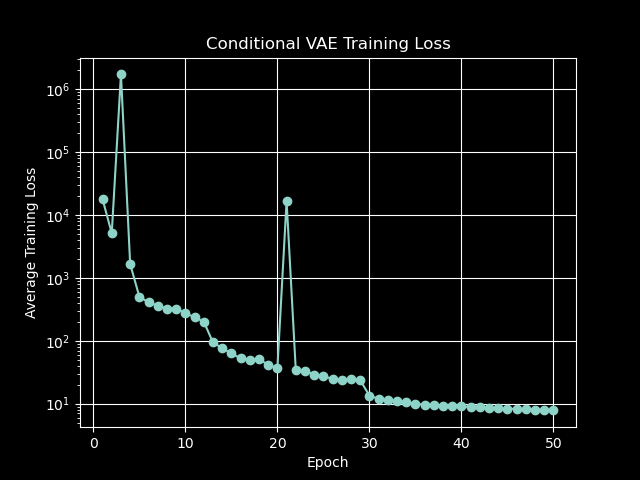
\includegraphics[width=0.6\textwidth]{../loss/cond_vae_loss_curve_20250321-061452.png}
    \caption{Training and loss showing the convergence of the conditional VAE model.}
    \label{fig:cond_vae_loss}
\end{figure}

\FloatBarrier

\paragraph{Autoregressive Prediction.}
After training, we predict multiple future steps by iteratively feeding the model’s own predictions back as input conditions. Specifically, if \(\hat{X}(t+1)\) is the model’s prediction given \(X(t)\), we then predict \(\hat{X}(t+2)\) by feeding \(\hat{X}(t+1)\) into the condition encoder. This is repeated for as many steps as needed.

\paragraph{Evaluation.}
We compare the predicted fields against the ground truth from 1985. Below are examples of the MSE curves and channel-wise predictions:

\begin{figure}[ht]
    \centering
    \begin{subfigure}[b]{0.4\textwidth}
        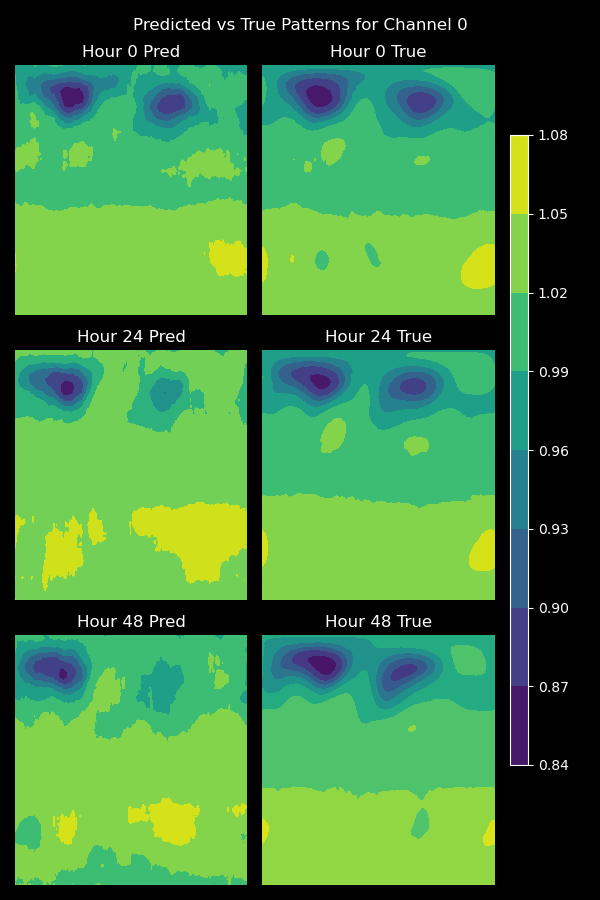
\includegraphics[width=\textwidth]{../plots/autoregressive_predictions_channel0_20250321-061452.png}
        \caption{Channel 0 predictions}
    \end{subfigure}
    \begin{subfigure}[b]{0.4\textwidth}
        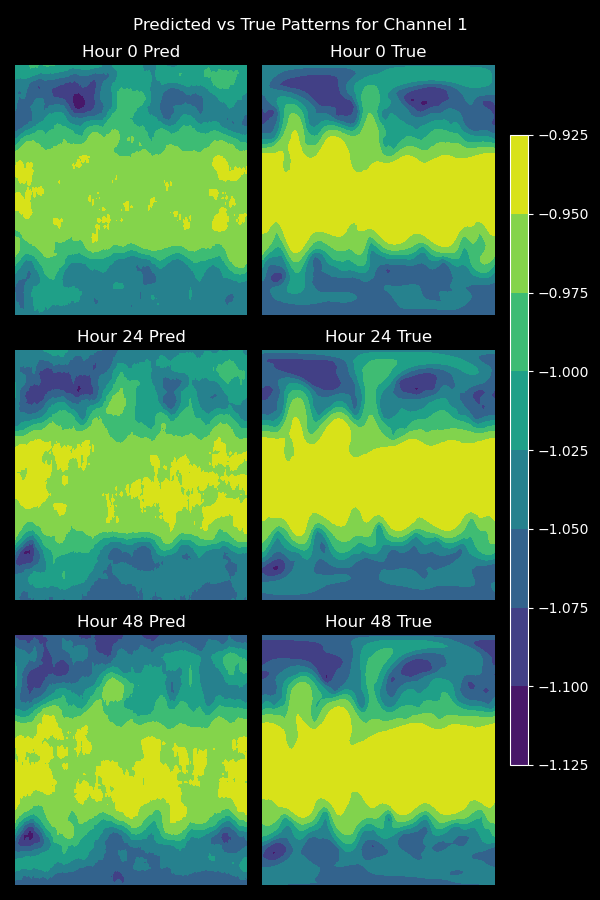
\includegraphics[width=\textwidth]{../plots/autoregressive_predictions_channel1_20250321-061452.png}
        \caption{Channel 1 predictions}
    \end{subfigure}
    \caption{Autoregressive predictions for both channels showing the model's ability to forecast multiple time steps ahead.}
    \label{fig:autoregressive_preds}
\end{figure}

\begin{figure}[ht]
    \centering
    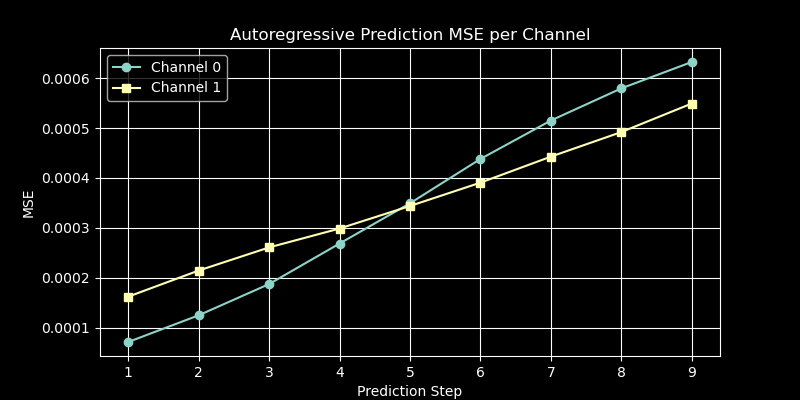
\includegraphics[width=0.5\textwidth]{../plots/autoregressive_mse_20250321-061452.png}
    \caption{Mean squared error over multiple autoregressive prediction steps, showing how prediction accuracy evolves with increasing time horizon.}
    \label{fig:autoregressive_mse}
\end{figure}

\FloatBarrier

\newpage
\section*{3 Problem (10 points)}

The forward diffusion process in a diffusion model is given by $q\left(x_t \mid x_{t-1}\right)$:
\[
x(t)=\sqrt{\left(1-\beta_t\right)} x(t-1)+\sqrt{\beta_t} \mathcal{N}(0, \mathbf{I})
\]
Prove that \(q\bigl(x_t \mid x_{t-1}\bigr)\) converges to a unit Gaussian as \(t \to \infty\) if \(\beta_t\) is constant in time. 

\paragraph{Proof:}
We consider the forward diffusion process defined by
\begin{equation}
  x_t = \sqrt{1-\beta}\, x_{t-1} + \sqrt{\beta}\, \epsilon_t, \quad \epsilon_t \sim \mathcal{N}(0, \mathbf{I}),
  \label{eq:diffusion}
\end{equation}
where $\beta \in (0,1)$ is constant in time. Our goal is to prove that the \emph{marginal} distribution of $x_t$, denoted $q(x_t)$, converges to the unit Gaussian distribution $\mathcal{N}(0, \mathbf{I})$ as $t \to \infty$.

\subsection*{Step 1: Expansion of the Process}

Starting from Equation~\eqref{eq:diffusion}, we can unroll the recurrence:
\[
\begin{aligned}
  x_t &= \sqrt{1-\beta}\, x_{t-1} + \sqrt{\beta}\, \epsilon_t,\\[1mm]
      &= \sqrt{1-\beta}\left(\sqrt{1-\beta}\, x_{t-2} + \sqrt{\beta}\, \epsilon_{t-1}\right) + \sqrt{\beta}\, \epsilon_t,\\[1mm]
      &= (1-\beta)^{t/2} x_0 + \sqrt{\beta}\sum_{s=1}^{t} (1-\beta)^{\frac{t-s}{2}} \epsilon_s.
\end{aligned}
\]
Since each $\epsilon_s$ is an independent standard Gaussian vector, $x_t$ is a linear combination of independent Gaussian random variables and is hence Gaussian.

\subsection*{Step 2: Mean Evolution}

Taking the expectation on both sides, and assuming $x_0$ is deterministic or has mean zero, we have
\[
\mathbb{E}[x_t] = (1-\beta)^{t/2} \, \mathbb{E}[x_0].
\]
Thus, if $\mathbb{E}[x_0] = 0$, then
\[
\mathbb{E}[x_t] = 0 \quad \text{for all } t.
\]
Even if $\mathbb{E}[x_0] \neq 0$, the factor $(1-\beta)^{t/2}$ tends to zero as $t \to \infty$, so the mean of $x_t$ converges to $0$.

\subsection*{Step 3: Variance Evolution}

Next, we compute the covariance of $x_t$. Since the noise terms are independent with covariance $\mathbf{I}$, the variance contribution from each noise term is scaled by the square of its coefficient:
\[
\begin{aligned}
\mathrm{Var}(x_t) &= \beta \sum_{s=1}^{t} \left((1-\beta)^{\frac{t-s}{2}}\right)^2 \, \mathbf{I}\\[1mm]
&= \beta \sum_{s=1}^{t} (1-\beta)^{t-s} \, \mathbf{I}\\[1mm]
&= \beta \sum_{k=0}^{t-1} (1-\beta)^k \, \mathbf{I}.
\end{aligned}
\]
Recognize that the sum is a geometric series:
\[
\sum_{k=0}^{t-1} (1-\beta)^k = \frac{1-(1-\beta)^t}{\beta}.
\]
Thus,
\[
\mathrm{Var}(x_t) = \beta \cdot \frac{1-(1-\beta)^t}{\beta} \, \mathbf{I} = \Bigl[1-(1-\beta)^t\Bigr] \, \mathbf{I}.
\]
As $t \to \infty$, $(1-\beta)^t \to 0$, so the covariance converges to $\mathbf{I}$.

\subsection*{Step 4: Convergence to the Unit Gaussian}

Since $x_t$ is Gaussian with mean
\[
\mathbb{E}[x_t] \to 0
\]
and variance
\[
\mathrm{Var}(x_t) \to \mathbf{I}
\]
as $t \to \infty$, we conclude that
\[
q(x_t) \xrightarrow{t\to\infty} \mathcal{N}(0, \mathbf{I}).
\]
proving that the marginal distribution of $x_t$ converges to a unit Gaussian distribution.


\end{document}